\documentclass[]{marticle}
\usepackage[utf8]{inputenc}
\usepackage[italian]{babel}
\usepackage{amssymb}
\usepackage{mstyle}

\title{\textbf{\Huge Relazione di Laboratorio Computazionale}}
\date{}


\begin{document}
\maketitle

\textbf{QUESTA \`E UNA BOZZA!}

\section*{Abstract}
In questa relazione prenderemo in considerazione il problema di estrarre
campioni di valori casuali data una certa distribuzione di probabilita` discreta.
Supporremo di sapere generare variabili uniformi sull'intervallo $[0,1]$, che
verranno implementate operativamente come le variabili generate dalla libreria
\code{numpy}.

Una prima soluzione del problema \`e quella di dividere $[0,1]$ in intervalli di
lunghezza pari a ciascuna componente del vettore di probabilit\`a, e scegliere
il risultato in funzione dell'intervallo a cui appartiene una variabile
uniforme. Questo presenta diversi inconvenienti: il metodo infatti richiede un
numero di somme proporzionale al numero di componenti del vettore di
probabilit\`a. Questo potrebbe essere intrattabile quando molto grande. Inoltre
spesso il vettore di probabilit\`a \`e noto solo a meno di un coefficiente di
normalizzazione, il cui calcolo richiederebbe di nuovo $O(n)$ somme. 

Uno dei metodi pi\`u utilizzati per ovviare a questi problemi \`e il metodo di
Monte Carlo (abbreviato spesso con MCMC, Markov Chain Monte Carlo), che consiste
nella simulazione di una camminata su una catena di Markov con distribuzione
invariante la distribuzione data. Dopo un numero sufficiente di step, la
frequenza di visita di un nodo sar\`a arbitrariamente vicina a quella voluta. In
questo caso per\`o il numero di passi necessari ad una determinata distribuzione
non \`e noto a priori ed \`e di difficile calcolo.

Si andr\`a dunque a presentare l'algoritmo di Propp-Wilson, una modifica del
MCMC che ha il vantaggio di ottenere la distribuzione esatta e di terminare una
volta raggiunta questa. Applicheremo tale algoritmo al modello di Ising, una
modellizzazione del comportamento magnetico della materia.

\section{Il modello di Ising}
In queste prime sezioni si segue l'approccio di \cite{bremaud}.

Sia $G=(V,E)$ un grafo non orientato. Considereremo dunque l'arco $(x,y)$ uguale
all'arco $(y,x)$. I vertici andranno a rappresentare i singoli atomi di un
materiale, e gli archi indicano quali atomi interagiscono fra loro. Ad ogni
atomo viene quindi associato uno spin che pu\`o essere $+1$ o $-1$. Una
configurazione \`e quindi una funzione $\sigma\colon V \rightarrow \{+1, -1\}$.
Chiameremo $\Sigma$ lo spazio di tali configurazioni.  A ciascuno di questi
modelli si associa l'energia 
\[
    H(\sigma) = -\sum_{(x,y)\in E} \sigma(x)\sigma(y).
\]
Inoltre viene dato un parametro reale del sistema $\beta \geq 0$ detta
temperatura inversa. Il modello di ising associa ad ogni configurazione $\sigma
\in \Sigma$ la probabilit\`a
\[
    \pi(\sigma) = \frac{1}{Z} \exp(-\beta H(\sigma))
\]
Dove $Z$ \`e il coefficiente di normalizzazione pari a
\[
    Z = \sum_{\sigma \in \Sigma} \exp(-\beta H(\sigma))
\]

L'obiettivo che ci prefiggiamo \`e quello di estrarre un campione da
$\Sigma$ con probabilit\`a $\pi$.

\section{Metodo di Monte Carlo}

Come prima cosa, data una distribuzione $\pi$ su un insieme $\Omega$, cerchiamo
una matrice di transizione $P$ per una catena di Markov omogenea che abbia
$\pi$ come misura invariante. Per farlo chiediamo una condizione pi\`u forte su
$P$, cio\`e la reversibilit\`a, ovvero si vuole che $\pi (i)P_{i,j}=\pi
(j)P_{j,i}$. Se la matrice $P$ \`e irriducibile e aperiodica, data una
distribuzione iniziale $\pi_0$, la distribuzione di probabilit\`a dopo $n$ passi
$\pi_n = \pi_0 P^n$ converge a $\pi$.

Cerchiamo allora le matrici del tipo $P_{i,j} = A_{i,j} Q_{i,j}$ per $i\neq j$,
dove la matrice $Q$ \`e irriducibile e viene detta matrice generatrice dei
candidati, e $A$ \`e da determinare in modo tale che $P$ abbia le propriet\`a
richieste e $0\leq A \leq 1$. Le componenti $P_{i,i}$ sono determinate in
maniera tale che $P$ sia stocastica.  A livello di interpretazione si pu\`o
pensare che a ogni step si sceglie vertice candidato a cui passare con
probabilit\`a dettata da $Q$ e poi si esegue il passagio con probabilit\`a
dettata da $A$, altrimenti si rimane nel vertice di partenza. Per questo motivo
$A$ \`e la matrice delle probabilit\`a di accettazione. 

Generalmente si sceglie $A$ della forma
\[
    A_{i,j} = \frac{S_{i,j}}{1+T_{i,j}}
\]
con
\[
    T_{i, j} = \frac{\pi(i) Q_{i,j}}{\pi(j) Q_{j,i}}
\]
e $S$ una matrice simmetrica.
L'algoritmo di Metropoli-Hastings sceglie
\[
    A_{i,j} = \min \left(1, \frac{\pi(i)Q_{j,i}}{\pi(j)Q_{i,j}}\right).
\]
 In questo modo si determina una $P$ con tutte le propriet\`a richieste.

\section{Il Gibbs sampler}

Vogliamo specializzare il MCMC ai casi in cui l'insime degli stati sia un
insieme di funzioni (con dominio e codominio finiti). Questa capita nel modello
di Ising che studieremo in seguito, per esempio. Abbiamo dunque un processo
stocastico a valori in $E=\Lambda^V$ per certi insiemi $\Lambda$ e $V$. 

Con il Gibbs sampler il processo passa da uno stato $X_n=f$ a $X_{n+1}=g$ con le
seguenti regole: sia $v$ un elemento scelto in modo casuale uniforme da $V$.
Allora $f$ e $g$ devono coincidere su $V\setminus\setof{v}$. Il punto $g(v)$
assume il valore $\lambda$ con probabilit\`a $\prob{X(v)=g(v) \ |\ X(v')=f(v')
\text{ per } v' \in V\setminus\setof{v}}$. Si verifica che la distribuzione
cercata soddisfa la condizione di reversibilit\`a e che la catena risultante \`e
irriducibile e aperiodica. Dunque si ha la converganza del metodo di Monte
Carlo.

In particolare il Gibbs sampler \`e un caso particolare del MCMC con
Metropoli-Hastings. In effetti scegliamo la matrice dei candidati $Q$ con le
probabili\`a sopra definite. A queto punto si verifica che tutte le entrate di
$A$ sono pari a $1$, e dunque $P=Q$.

\section{Coupling from the past}

In questa sezione svilupperemo un metodo per estrarre un campione con una
probabilit\`a esatta $\pi$, data $P$ una matrice di transizione irriducibile e
aperiodica su un insieme finito di stati $S=\setof{s_1,\dots,s_n}$ e con
probabilit\`a invariante $\pi$. Possiamo associare alla catena di Markov
definita da $P$ una funzione di transizione 
\[
    f\colon S\times [0,1] \longrightarrow S
\]
tale che se $U$ \`e una variabile uniforme sull'intervallo $[0,1]$, allora 
\[
    \prob{f(s_i,U)=s_j}=P_{i,j} \qquad \forall s_i,s_j \in S.
\]

Siano $U_m$ variabili uniformi su $[0,1]$ per ogni $m\in \Z$. Costruiamo allora
delle sequenze $X^r_m(i)$ con $i = 1,\dots,n$, $r\leq 0$ e $m \geq r$ interi nel
modo seguente:
\[
    X^r_r(i) = s_i
\]
\[
    X^r_{m+1}(i) = f(X^r_m(i), U_m).
\]

Sia ora 
\[
    \tau^-=\min(\ -r \st X^r_0(1) = \dots = X^r_0(n))
\]
e definiamo $Y = X^{\tau^-}_0(1)$. La condizione con cui \`e stato definito
$\tau^-$ \`e detta coalescenza e $\tau^-$ \`e detto tempo di accoppiamento
all'indietro.

Si verifica che $Y$ ha distribuzione pari a $\pi$.

Questo metodo \`e noto come algoritmo di Propp-Wilson \cite{propp-wilson}.

In figura \ref{fig:im1} c'\`e un esempio di una simulazione con Propp-Wilson. Il
tempo di coalescenza all'indietro \`e 6, e la variabile $Y$ avr\`a il valore
dello stato centrale. Si noti che una volta che due catene assumono lo stesso
valore, esse rimangono unite da quel punto in poi.

\begin{figure}[h!]
\input{images/pw_coal.pdf_tex}
\caption{Esempio di catene generate con Propp Wilson.}
\label{fig:im1}
\centering
\end{figure}


\textit{Esempio.} Proviamo a descrivere una semplificazione dell'algoritmo di
Propp-Wilson e descriviamo un esempio per cui essa non funziona. Come sopra
prendiamo le $U_m$ variabili indipendenti uniformi sull'intervallo unitario con
$m$ che varia sui numeri naturali. Consideriamo le $n$ catene $X(i)$ in modo
simile a prima, partendo per\`o da 0, ovvero
\[
    X_0(i) = s_i
\]
e
\[
    X_{m+1}(i) = f(X_m(i), U_m).
\]
Consideriamo il tempo di accoppiamento nel futuro
\[
    \tau^+ = \min(\ m \st X_m(1) = \dots = x_m(n)\ )
\]
e il rispettivo stato $Y = X_{\tau^+}(1)$. In questo caso per\`o $Y$ non ha la
distribuzione $\pi$ richiesta. 
Per farlo vedere prendiamo l'insieme degli stati composto da due elementi $S =
\setof{s_1, s_2}$ e la seguente matrice di transizione:
\[
    P = 
    \begin{pmatrix}
        0.5 & 0.5 \\
        1  & 0
    \end{pmatrix}.
\]
La catena ha probabilit\`a invariante $\pi = (\frac{2}{3}, \frac{1}{3})$. Per
definizione, le due catene al tempo $\tau^+$ si trovano nello stesso stato, e al
tempo $\tau^+-1$ si trovano una in $s_1$ e l'altra in $s_2$. La seconda allora
al passo $\tau^+$ deve andare in $s_1$ con probabilit\`a $1$. Quindi con questo
algoritmo, $Y=s_1$ quasi certamente.

Pensando all'algoritmo, a priori dovremmo simulare la catena $X^{-1}$, vedere se
si ha la coalescenza, e in caso negativo simulare $X^{-2}$ e procedere in
maniera analoga. Questo richiederebbe in effetti il calcolo di un numero di step
della catena di Markov pari a $1+\dots+\tau^- = O((\tau^-)^2)$. Notiamo per\`o
che se $r'>\tau^-$ si ha che $X^{r'}_0(i) = Y$. Questo rende possibile calcolare
le catene $X^{-2^k}$ ottenendo lo stesso risultato. Il numero di step richiesto
in questo caso \`e $2^0+2^1 + \dots + 2^c$ dove $c$ \`e il pi\`u piccolo intero
tale che $2^c \geq \tau^-$, in particolare si ha $2^c < 2\tau^-$. La somma viene
dunque maggiorata da $4\tau^-$, un costo decisamente vantaggioso rispetto al
precedente.

\section{Sandwiching}

Il metodo presentato sopra \`e funzionante e risolve gli scopi che ci eravamo
prefissi, tuttavia simulare tutte le $n$ catene di Markov \`e praticamente
impossibile per $n$ grandi. In questa sezione ci occuperemo di migliorare il
metodo per renderlo computazionalmente pi\`u leggero.
 
In questo caso supporremo di avere un ordine parziale tra gli stati in $S$ che
denoteremo con il simbolo $\preceq$. Richiediamo che la funzione di transizione
rispetti la condizione di monotonia
\[
    f(s_i, u) \leq f(s_j, u) \qquad \forall s_i \preceq s_j,\ u \in [0,1]
\]

e che esistano in $S$ un massimo e un minimo, che senza perdita di generalit\`a
chiameremo $s_1$ e $s_n$. Si verifica facilmente che la coalescenza di $X^r_0$
si verifica se e solo se $X^r_0(1) = X^r_0(n)$. In figura \ref{fig:im2} si ha un
esempio di queste catene. In questo caso il tempo di coalescenza \`e 7.

\begin{figure}[h!]
\input{images/mon_coal.pdf_tex}
\caption{Esempio di catene monotone generate con Propp Wilson.}
\label{fig:im2}
\centering
\end{figure}

Questa idea \`e efficace perch\'e il tempo di coalescenza $\tau^-$ \`e quasi
certamente finito e la variabile $Y=X^{\tau^-}_0(1)$ ha distribuzione $\pi$.

\textit{Dimostrazione.} Notiamo come prima cosa che il tempo $\tau^+$ (definito
come nell'esempio sopra) \`e dominato dal primo $m$ positivo per cui $X_m(n) =
s_1$. Questo $m$ \`e finito perch\'e la catena di Markov in considerazione \`e
ergodica. 

Ora mostriamo che per ogni $k$ naturale si ha che $\prob{\tau^- \leq k} =
\prob{\tau^- \leq k}$. Consideriamo la successione di valori casuali per
valutare gli step $U_m$, e trasliamola indietro di $k$ posizioni, cio\`e
prendiamo $U'_m = U_{m-k}$. Sia $\tau'$ il tempo di accopiamento all'indietro
realtivo alla successione $U'$. Ovviamente si ha che $\tau'$ e $\tau^-$ sono
variabili identicamente distribuite. Supponiamo che valga $\tau^+ \leq k$.
Allora nel modello degli $U'$ si ha la coalescenza al tempo $\tau^+ - k  \leq
0$, e quindi abbiamo trovato che $\tau' \leq k$. Dunque
\[
    \prob{ \tau^+ \leq k} \leq \prob{ \tau' \leq k} = \prob{ \tau^- \leq k}.
\]
Viceversa prendiamo $\tau' \leq k$. Ragionando in modo analogo a prima,
otteniamo che la catena originaria ha coalescnza in avanti prima del tempo $k$,
e si ha la disuguaglianza opposta.

Mettendo assieme i due pezzetti si trova che $\tau^-$ \`e quasi certamente
finito. 

Verifichiamo ora la distribuzione di $Y$. Per $r \geq \tau^-$ vale
\begin{align*}
    \prob{Y=j} =&\ \prob{Y=j,\ \tau^- > n} + \prob{Y=j,\ \tau^- \leq n} \\
    =&\ \prob{Y=j,\ \tau^- > n} + \prob{X_0^r(i)=j,\ \tau^- \leq n} \\
    =&\ \prob{Y=j,\ \tau^- > n} - \prob{X_0^r(i)=j,\ \tau^- > n} 
            + \prob{X_0^r(i)=j} \\
    =&\ A_n - B_n + P^n_{i,j}.
\end{align*}

Gli $A_n$ e $B_n$ sono limitati dall'alto da $\prob{\tau^- > n}$, che \`e una
quantit\`a che tende a zero per $n$ grande perch\`e il tempo di accoppiamento
\`e quasi certamente finito. L'ultimo termine tende invece alla probabilit\`a
invariante e questo conclude la dimostrazione.


\section{Implementazione del modello di Ising}
Andiamo ad utilizzare le tecnice viste al modello di Ising, sviluppando gli
esercizi 11.3 e 11.4 di \cite{haggstrom}. Innanzi tutto ci ridurremo al caso in
cui il grafo \`e una griglia quadrata di lato $l$. Sui possibili stati di un
grafo, consideriamo la relazione d'ordine definita da: $\sigma \preceq \xi$ se e
solo se per ogni vertice $v$ si ha che $\sigma(v) \leq \xi(v)$.  Con questa
realzione si hanno due stati particolari, le due funzioni costanti, che sono il
massimo e il minimo. Lo scopo \`e quello di simulare le catene di Markov che
partono da questi stati. 

Sia $\xi$ una possibile configurazione sul grafo $(V,E)$. Sia inoltre $v$ un
vertice e consideriamo le configurazioni $\xi_p$ e $\xi_n$ che sono uguali a
$\xi$ in tutti i punti tranne $v$, dove valgono rispettivamente $+1$ e $-1$.
Andiamo allora a calcolare il rapporto
\begin{align*}
    \frac{\pi(\xi_p)}{\pi(\xi_n)} =& 
    \frac{\exp (\beta \sum_{(y,z)\in E} \xi_p(y)\xi_p(z))} {\exp
            (\beta\sum_{(y,z)\in E} \xi_n(y)\xi_n(z))} \\
    =& \exp \left[\beta\sum_{(y,z)\in E}
        \left(\xi_p(y)\xi_p(z)-\xi_n(y)\xi_n(z)\right)\right ]\\
    =& \exp \left[\beta\sum_{(v,y)\in E}
        \left(\xi_p(v)\xi_p(y)-\xi_n(v)\xi_n(y)\right)\right ]\\
    =& \exp \left[\beta\sum_{(v,y)\in E}
        \left(\xi_p(v)-\xi_n(v)\right)\xi(y)\right ]\\
    =& \exp \left[2\beta\sum_{(v,y)\in E} \xi(y)\right ]
    = \exp \left(2\beta\kappa(\xi,v)\right)
\end{align*}
dove $\kappa(f,x)$ indica la somma di tutti i valori di $f$ nei vertici
adiacenti a $x$.

Sia $X$ una variabile aleatoria con la distribuzione del modello di Ising.
Andiamo allora a calcolare la probabilit\`a condizionale del Gibbs sampler.
\begin{align*}
    \eta(\xi,v) =&
    \prob{X(v)=+1\ |\ X(V\setminus \setof{v}=\xi}\\
    =& \frac{\pi(\xi_p)}{\pi(\xi_p)+\pi(\xi_n)}
    = \frac{\exp(2\beta\kappa(\xi,v))}{\exp(2\beta\kappa(\xi,v))+1}
\end{align*}

Dunque per compiere uno step nella catena di Markov partendo da uno stato $X_m$,
si sceglie uniformemente un vertice $v$ e lo si pone a $+1$ con probabilit\`a
$\eta(X_n, v)$. Cio\`e si prende una variabile uniforme sull'intervallo unitario
$U_m$ e si pone $v$ a $+1$ se $U_m<\eta(X_m,v)$. Definiamo la funzione di
aggiornamento
\[
    \Phi(\xi, u)(v) = 
    \begin{cases}
        +1 \text{\quad se $u < \eta(\xi,v)$}\\
        -1 \text{\quad altrimenti}
    \end{cases}
\]
e $\Phi(\xi,u)(w) = \xi(w)$ per tutti i vertici $w$ diversi da $v$.

Al fine di avvantaggiarci con la tecnica del sandwiching, bisogna ancora
verificare che queste operazioni conservano l'ordine parziale. Prendiamo quindi
$\xi \preceq \xi'$ due possibili stati, un vertice $v$ e un reale $u\in[0,1]$.
Notiamo intanto che
\[
    \kappa(\xi,v) = \sum_{(v,y)\in E} \xi'(y) \leq
    \sum_{(v,y)\in E} \xi(y) = \kappa(\xi', v).
\]
Ne segue che 
\[
    \eta(\xi,v) = \frac{\exp(2\beta\kappa(\xi,v))}{\exp(2\beta\kappa(\xi,v))+1}
    \leq \frac{\exp(2\beta\kappa(\xi',v))}{\exp(2\beta\kappa(\xi',v))+1}
    = \eta(\xi',v)
\]
e dunque si ha anche la monotonia di $\Phi$ nel primo argomento.

Si fornisce in seguito l'implementazione dell'algoritmo descritto in Python. In
particolare la funzione \texttt{get\_ising} accetta un intero \texttt{N} e il
valore \texttt{beta} e restituisce una matrice con un campione del modello di
Ising sul grafo fatto come una griglia quadrata di lato \texttt{N}.

\begin{lstlisting}
import numpy as np
import numpy.random as rnd

# Questa classe si occupa di produrre e ricordare i valori casuali
class Random_gen:
    def __init__(self, N):
        self.N = N
        self.depth = 0
        self.rarr = np.zeros((0,), dtype=float)
        self.narr = np.zeros((0,2), dtype=int)

    def advance_depth(self, nd):
        self.rarr.resize((nd,))
        self.narr.resize((nd,2))
        diff = nd - self.depth
        self.rarr[self.depth:] = rnd.random((diff,))
        self.narr[self.depth:] = rnd.randint(0, self.N, size=(diff,2))
        self.depth = nd

def multiple_step(M, beta, rarr, narr):
    n = rarr.size
    for i in range(n):
        index = n - i - 1
        r = rarr[index]
        x = narr[index,0]
        y = narr[index,1]
        acc = 0
        if x > 0:
                acc += M[x-1,y]
        if y > 0:
                acc += M[x,y-1]
        if y < N-1:
                acc += M[x,y+1]
        if x < N-1:
                acc += M[x+1,y]
        a = np.exp( 2 * beta * acc )
        u = a / (a+1)
        if r < u:
            M[x, y] = 1
        else:
            M[x, y] = -1

def get_ising(N, beta):
    depth = 1
    ran = Random_gen(N)
    ran.advance_depth(depth)
    while True:
        up = np.ones((N,N), dtype=int)
        down = np.full((N,N), -1, dtype=int)
        multiple_step(up, beta, ran.rarr, ran.narr)
        multiple_step(down, beta, ran.rarr, ran.narr)
        # Verifica se si ha la coalescenza
        if np.array_equal(up, down): 
            break
        else:
            depth = max(depth+1, depth*2)
            ran.advance_depth(depth)
    return up
\end{lstlisting}

Provando a fare girare il programma a diversi valori di $\beta$ e della
dimensione della griglia, notiamo, come mostrato in figura \ref{fig:plot1} che i
tempi di attesa diventano molto lunghi per la temperatura inversa che si
avvicina a $0.4$. In particolare notiamo che la crescita del numero di step
necessari alla coalescenza \`e circa esponenziale in $\beta$. Per ovviare a
questo problema, che a livello pratico impedisce alla computazione di terminare
per molti valori dei parametri, nella prossima sezione si presenter\`a un
miglioramento del metodo.

\begin{figure}[h!]
\caption{Numero di step richiesti per la coalescenza per una griglia di lato 10.}
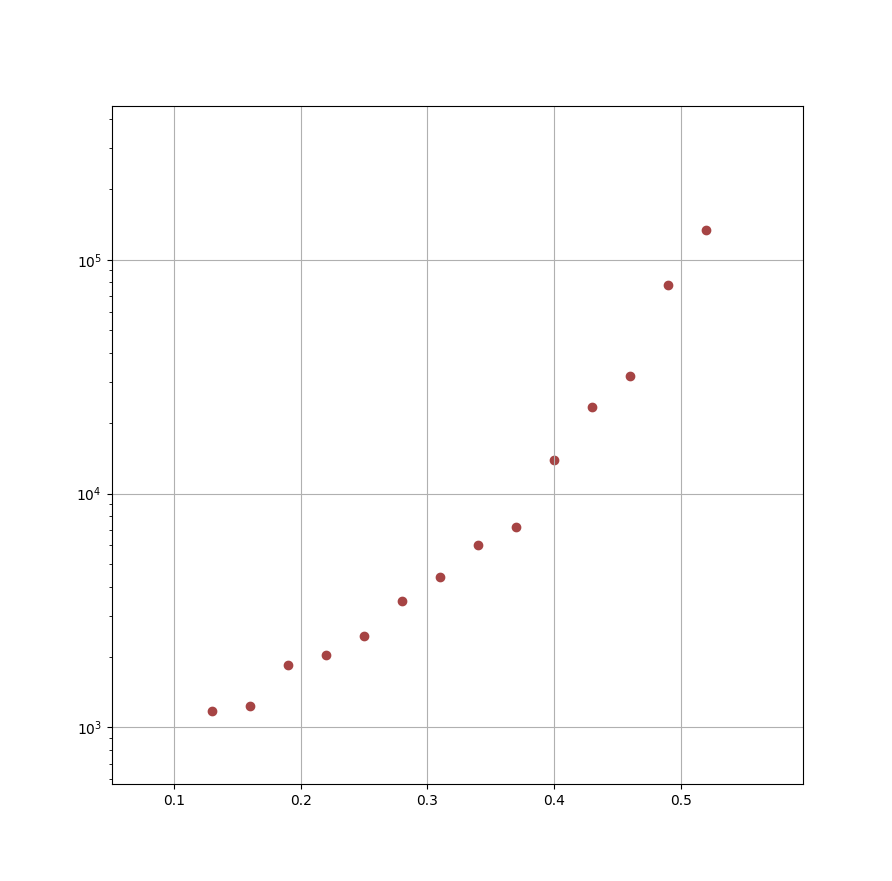
\includegraphics[width=\textwidth]{pp_times_10}
\label{fig:plot1}
\centering
\end{figure}

\section{Random Cluster}
I seguenti risultati sono stati ottenuti sviluppando la traccia in
\cite{edwards-sokal}.

Consideriamo un grafo non orientato $G=(V,E)$, sia poi $\Sigma$ lo spazio delle
possibili configurazioni di un modello di Ising su $G$, ossia $\setof{0,1}^V$.
Siano inoltre $\Omega$ l'insieme dei sottografi di $G$, che identificheremo
anche con l'insieme delle parti di $E$, e $\bar{\omega}\colon \Sigma
\longrightarrow \Omega$ la funzione tale che 
\[
    \bar{\omega}(\sigma) = \setof{(i,j)\in E \st \sigma(i) = \sigma(j)}
\]
e che associa ad ogni configurazione $\sigma$ il pi\`u grande sottografo di $G$
tale per cui $\sigma$ \`e costante sulle sue componenti connesse.

Consideriamo la distribuzione di probabilit\`a definita su $\Sigma \times
\Omega$ come
\[
    \mu_p(\sigma, \omega) = \frac{1}{Z_{FK}} p^{|\omega|} (1-p)^{|E| - |\omega|}
    \ind(\omega \subseteq \bar{\omega})
\]
dove $Z_{FK}$ \`e un opportuno coefficiente di normalizzazione e $\ind$ vale $1$ se
e solo se il suo argomento \`e vero e $0$ altrimenti.

Calcoliamo le distribuzioni marginali su $\Omega$ e $\Sigma$.
\begin{align*}
    \mu^1_p(\sigma) =& \sum_{\omega\in\Omega} \mu_p(\sigma,\omega) = 
    Z_{FK}^{-1} \sum_{\omega\subseteq\bar{\omega}(\sigma)}  p^{|\omega|}
    (1-p)^{|E| - |\omega|} \\
    =& Z_{FK}^{-1} \sum_{k=0}^{|\bar{\omega}(\sigma)|}
        \binom{|\bar{\omega}(\sigma)|}{k}
        p^k (1-p)^{|E| - k} \\
    =& Z_{FK}^{-1} (1-p)^{|E|-|\bar{\omega}(\sigma)|}
        \sum_{k=0}^{|\bar{\omega}(\sigma)|}  p^k
        \binom{|\bar{\omega}(\sigma)|}{k}
        (1-p)^{|\bar{\omega}(\sigma)| - k} \\
    =& Z_{FK}^{-1} (1-p)^{|E|-|\bar{\omega}(\sigma)|}
\end{align*}
Notiamo che vale
\[
    |\bar{\omega}(\sigma)| = \sum_{(x,y)\in E} \frac{\sigma(x) \sigma(y) +
    1}{2} = \frac{|E|}{2} - \frac{1}{2}H(\sigma)
\]
che ci permette di riscrivere
\[
    \mu^1_p(\sigma) = Z^{-1} \exp(-\beta H(\sigma))
\]
per $p = 1-e^{-2\beta}$ e per $Z$ che assorbe tutti i termini rimanenti (che non
dipendono da $\sigma$), ritrovando cos\`i la distribuzione del modello di Ising.

L'altra distribuzione marginale vale
\[
    \mu^2_p(\omega) = \nu(\omega) = \sum_{\omega\in\Omega} \mu_p(\sigma,\omega)
    = Z_{FK}^{-1} p^{|\omega|} (1-p)^{|E| - |\omega|} |\setof{\sigma \st
    \omega\subseteq\bar{\omega}(\sigma)}|
\]
Il numero di elementi di $\setof{\sigma \st
\omega\subseteq\bar{\omega}(\sigma)}$ \`e pari al numero di $\sigma$ costanti
sulle componenti connesse di $\omega$, cio\`e \`e il numero di possibili
assegnazioni di $+1$ o $-1$ a esse. Se indichiamo con $C(\omega)$ il numero di
componenti connesse di $\omega$,
\[
    \mu^2_p(\omega) = 
    Z_{FK}^{-1} p^{|\omega|} (1-p)^{|E| - |\omega|} 2^{C(\omega)}.
\]

Come ulteriore passo, ci serve ancora conoscere la probabilit\`a condizionata
$\mu_p[(\sigma,\omega)\ |\ (\cdot,\omega)]$, che vale 
\[
    \mu_p[(\sigma,\omega)\ |\ (\cdot,\omega)]
    = \frac{\ind(\omega \subseteq \bar{\omega})} {2^{C(\omega)}}.
\]
Per cui, conoscendo $\omega$, la configurazione $\sigma$ \`e scelta
uniformemente fra tutte le configurazioni costanti sulle componenti connesse di
$\omega$.

A questo punto abbiamo una strategia per trovare una configurazione del modello
di Ising con la distribuzione desiderata: si costruisce un sottografo $\omega$
con distribuzione $\nu$ con l'algoritmo di Propp-Wilson, poi ad ogni componente
connessa di esso si associa il valore $+1$ o $-1$ con probabilit\`a $1/2$. A
prima vista questa pu\`o sembrare una macchinosa complicazione, ma in realt\`a
l'implentazione con i cluster richiede molti meno step per la coalescenza.

\section{Implementazione con Random Cluster}

Identifichiamo gli elementi di $\Omega$ (sottoinsiemi di $E$) con le funzioni da
$E$ in  $\setof{0,1}$. Dati allora $\omega\in\Omega$ e $e\in E$, costruiamo
$\omega_p$, $\omega_n\in\Omega$ tali che essi concordano con $\omega$ su tutto
$E \setminus \setof{e}$, e inoltre $\omega_p(e) = 1$ mentre $\omega_n(e)=0$. 
Poich\`e $\omega_p$ e $\omega_n$ differiscono per un solo arco, o hanno lo
stesso numero di componenti connesse, o $\omega_p$ ha esattamente una componente
connessa in meno di $\omega_n$. Questo permette di calcolare agevolmente la
probabilit\`a condizionale del Gibbs sampler. Se $X$ \`e una variabile aleatoria
a valori in $\Omega$ e distribuzione $\nu$,
\[
    \prob{X=\omega_p \ |\ X(e')=\omega(e') \ \forall e' \neq e} = 
    \frac{\nu(\omega_p)}{\nu(\omega_p)+\nu(\omega_n)} = 
    \begin{cases}
        p \text{\quad se $C(\omega_p) \neq C(\omega_n)$}\\
        \frac{p}{2-p} \text{\quad altrimenti}.
    \end{cases}
\]

Notiamo che per $0<p<1$ vale che $\frac{p}{2-p}<p$, che, scelto uniformemente un
arco $e$, consente di costruire la funzione per lo step:
\[
    \Psi(\omega,u)(e) =
    \begin{cases}
        \omega \cup \setof{e} \text{\qquad se $u<\frac{p}{2-p}$}\\
        \omega \cup \setof{e} \text{\qquad se $u<p$ e $C(\omega_p) =
            C(\omega_n)$}\\
        \omega \setminus \setof{e} \text{\qquad altrimenti.} 

    \end{cases}
\]
Su tutti gli altri archi $\Psi(\omega)$ concorda con $\omega$.

Ordiniamo $\Omega$ per inclusione (questo ordine corrisponde a quello definito
su $\Sigma$ se visto $\Omega$ come insieme di funzioni) e verifichiamo la
monotonia di $\Psi$ nel suo primo argomento.

Vale intanto che se $\omega\subseteq\omega'$ e $C(\omega_p)=C(\omega_n)$ allora
$C(\omega'_p) = C(\omega'_n)$. Si distinguono allora i casi:
\begin{itemize}
    \item Se $u<\frac{p}{2-p}$ allora $\omega$ e $\omega'$ si aggiornano nello
        stesso modo.
    \item Se $u\geq p$ vale lo stesso ragionamento.
    \item Se $\frac{p}{2-p} \leq u < p$ e $\Psi(\omega') = \omega'_n$ allora
        $C(\omega'_p)\neq C(\omega'_n)$ e dunque $C(\omega_p)\neq C(\omega_n)$,
        concludendo che $\Psi(\omega) = \omega_n$. Cio\`e gli archi si
        aggiornano nello stesso modo.
    \item Se $\frac{p}{2-p} \leq u < p$ e $\Psi(\omega) = \omega_p$ allora si
        ragiona come nel caso precedente e si ottiene che gli archi si
        aggiornano nello stesso modo.
    \item In tutti i rimanenti casi vale che $\Psi(\omega')=\omega'_p$ e
        $\Psi(\omega)=\omega_n$.
\end{itemize}
In tutte le situazioni l'ordine viene mantenuto.

Per chiarezza si presenta lo pseudocodice per lo step della catena di Markov:
\begin{lstlisting}
def step(omega):
    e = random_edge() # Selezione casuale di un arco
    u = random() # Selezione casuale di un reale in [0,1]
    remove(omega, e) # Viene rimosso (se presente) l'arco
    if u < p/(2-p):
        insert(omega, e) # Si inserisce l'arco

    # are\_in\_the\_same\_component ritorna vero se e solo se 
    # gli estremi di e si trovano nella stessa componente
    # connessa di omega
    elif u < p and are_in_the_same_component(omega, e):
        insert(omega, e)
\end{lstlisting}

Nel codice che segue, \texttt{are\_in\_the\_same\_component} \`e implementato
attreverso una visita BFS della componente connessa di uno dei suoi vertici. Il
suo tempo \`e quindi dominato dalla dimensione dei cluster e quindi del numero
totale di vertici. 

Inoltre le configurazioni su $\Omega$ sono rappresentate come matrici $N\times N
\times 2$, con $N$ lato della griglia quadrata. L'elemento in posizione
$(i,j,d)$ rappresenta l'arco che parte dal vertice in $(i,j)$ e va alla sua
destra se $d=0$, immdiatamente verso il basso se $d=1$.

\begin{lstlisting}
import numpy as np
import numpy.random as rnd
from collections import deque


class Random_gen:
    def __init__(self, N):
        self.nmax = N * N * 2
        self.depth = 0
        self.rarr = np.zeros((0,), dtype=float)
        self.narr = np.zeros((0), dtype=int)

    def advance_depth(self, nd):
        self.rarr.resize((nd,), refcheck=False)
        self.narr.resize((nd,), refcheck=False)
        self.rarr[self.depth:] = rnd.random((nd-self.depth,))
        self.narr[self.depth:] = rnd.randint(0, self.nmax, size=(nd-self.depth,))
        self.depth = nd

def are_in_same_cc(V, x1, x2):
    que = deque()
    x = x1
    N = V.shape[0]
    adj = [(1,0,0),(0,1,1),(-1,0,0),(0,-1,1)]
    visited = np.zeros((N,N), dtype=bool)
    visited[x] = True
    while len(que) > 0:
        x = que.popleft()
        if x == x2:
            return True
        visited[x] = True
        (i,j) = x
        if i+1 < N and V[i,j,0] == 1 and visited[i+1, j] == 0:
            que.append((i+1, j))
        if j+1 < N and V[i,j,1] == 1 and visited[i, j+1] == 0:
            que.append((i, j+1))
        if i > 0 and V[(i-1,j,0] == 1 and visited[i-1, j] == 0:
            que.append((i-1, j))
        if j > 0 and V[i,j-1,1] == 1 and visited[i, j-1] == 0:
            que.append((i, j-1))
    return False

def multiple_step(p, V, narr, rarr):
    depth = rarr.size
    N = V.shape[0]
    for i in range(depth):
        index = depth - i - 1
        u = rarr[index]
        x = narr[index]
        i = x % N
        x = x // N
        j = x % N
        x = x // N
        d = x % 2
        e = (i,j,d)
        th1 = p / (2-p)
        if d == 0:
            y1 = 1
            y2 = 0
        else:
            y1 = 0
            y2 = 1
        x2 = ((i+y1)%N, (j+y2)%N)
        x1 = (i,j)
        V[i,j,d] = 0
        if u < th1:
            V[i,j,d] = 1
        elif u < p and are_in_same_cc(V, x1, x2):
            V[i,j,d] = 1

def get_clustered(N, p):
    depth = 1
    ran = Random_gen(N)
    ran.advance_depth(depth)
    while True:
        up = np.ones((N,N,2), dtype=bool)
        down = np.zeros((N,N,2), dtype=bool)
        multiple_step(p, up, ran.narr, ran.rarr)
        multiple_step(p, down, ran.narr, ran.rarr)
        if np.array_equal(up, down):
            break
        else:
            depth = max(depth+1, depth*2)
            ran.advance_depth(depth)
    return up

def get_ising(N, beta):
    p = (1 - np.exp(-beta*2))
    V = get_clustered(N, p)
    M = np.zeros((N,N), dtype=int)
    for i in range(N):
        for j in range(N):
            if M[i,j] != 0:
                continue
            sigma = rnd.randint(0,2) * 2 - 1
            que = deque()
            que.append((i,j))
            while len(que) > 0:
                i,j = que.popleft()
                M[i,j] = sigma
                if i+1 < N and V[i,j,0] == 1 and M[i+1, j] == 0:
                    que.append((i+1, j))
                if j+1 < N and V[i,j,1] == 1 and M[i, j+1] == 0:
                    que.append((i, j+1))
                if i > 0 and V[(i-1,j,0] == 1 and M[i-1, j] == 0:
                    que.append((i-1, j))
                if j > 0 and V[i,j-1,1] == 1 and M[i, j-1] == 0:
                    que.append((i, j-1))
    return M
\end{lstlisting}

Notiamo che con i random cluster, i tempi necessari alla coalescenza rimangono
stabili al veriare del parametro $\beta$, come mostrato in figura
\ref{fig:plot2}.

\begin{figure}[]
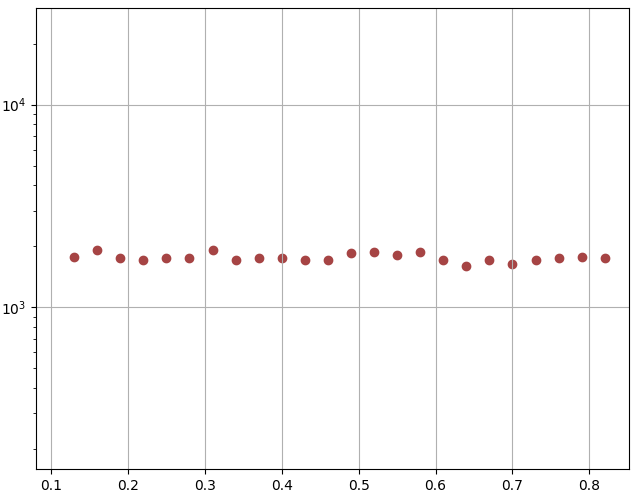
\includegraphics[width=\textwidth]{ff_times_10}
\caption{Numero di step richiesti per la coalescenza per una griglia di lato 10
    con i random cluster.}
\label{fig:plot2}
\centering
\end{figure}

\section{Transizione di fase} In figura \ref{fig:plot3} si mostrano diverse
configurazioni tipo a diverse temperature. Il punto colorato indica lo spin
$+1$. Si nota che man mano che la temperatura diminuisce, cio\`e man mano che
$\beta$ aumenta, si tendono a formare regioni pi\`u grandi di vertici orientati
nello stesso modo, e equivalentemente i cluster diventano pi\`u grandi. 

\begin{figure}[]
\begin{subfigure}{.5\textwidth}
  \centering
  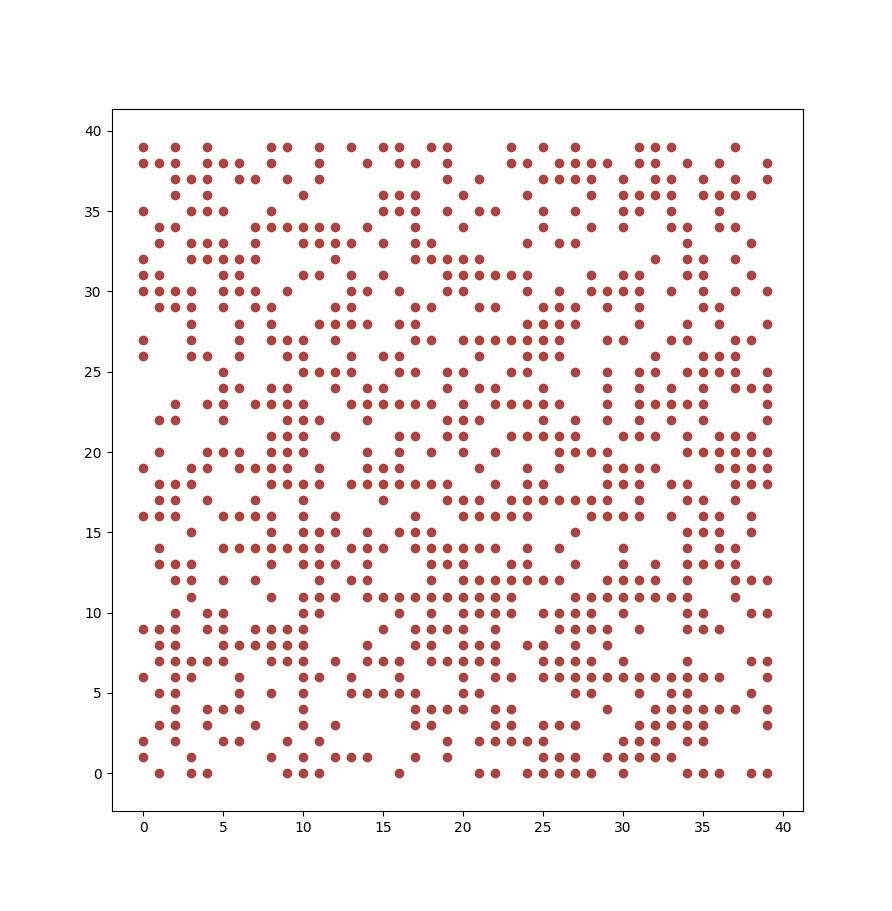
\includegraphics[width=.8\linewidth]{conf_40_0.0}
  \caption{$\beta$=0}
\end{subfigure}%
\begin{subfigure}{.5\textwidth}
  \centering
  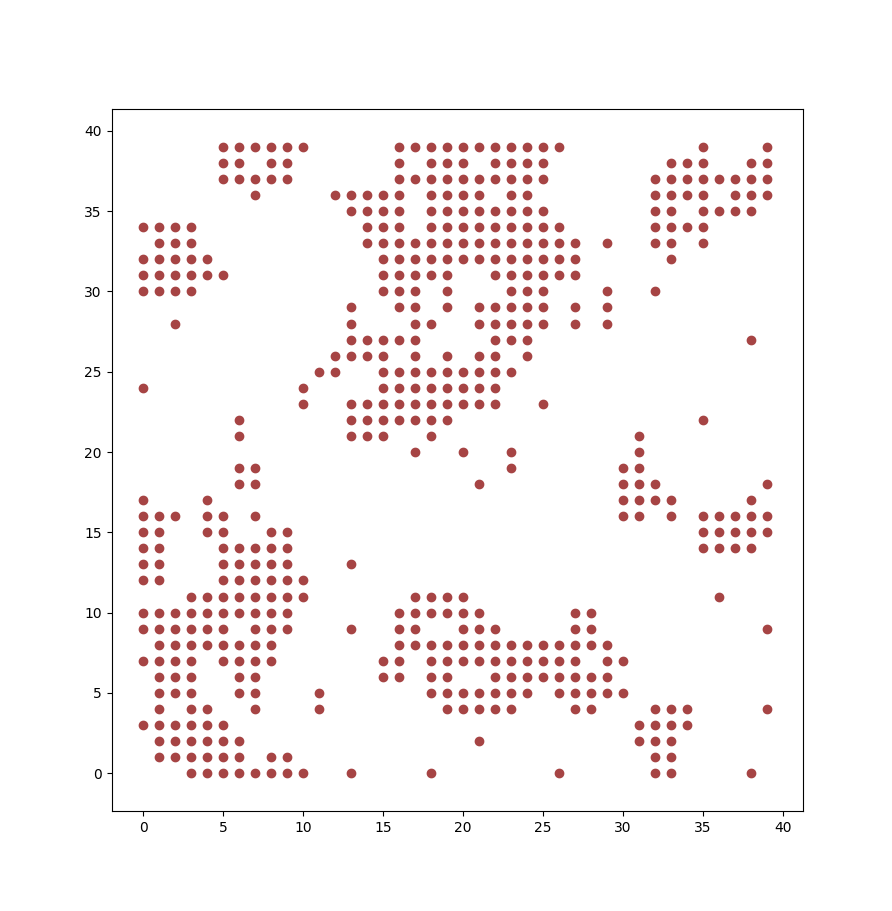
\includegraphics[width=.8\linewidth]{conf_40_0.5}
  \caption{$\beta$=0.5}
\end{subfigure}%
\caption{Configurazioni con $N=40$}
\label{fig:plot3}
\centering
\end{figure}

Per mostrare bene questo comportamento definiamo la magnetizzazione di una
configurazione $\sigma$ come il valore assoluto della somma di tutti gli spin
normalizzata sul numero di vertici. Andando a vedere come la magnetizzazione
cambia al variare di $\beta$ in figura figura \ref{fig:plot4}, si nota che si ha
una brusca salit\`a tra i valori 0.4 e 0.5. Tale cambio di comportamento \`e
detta transizione di fase. 

\begin{figure}[]
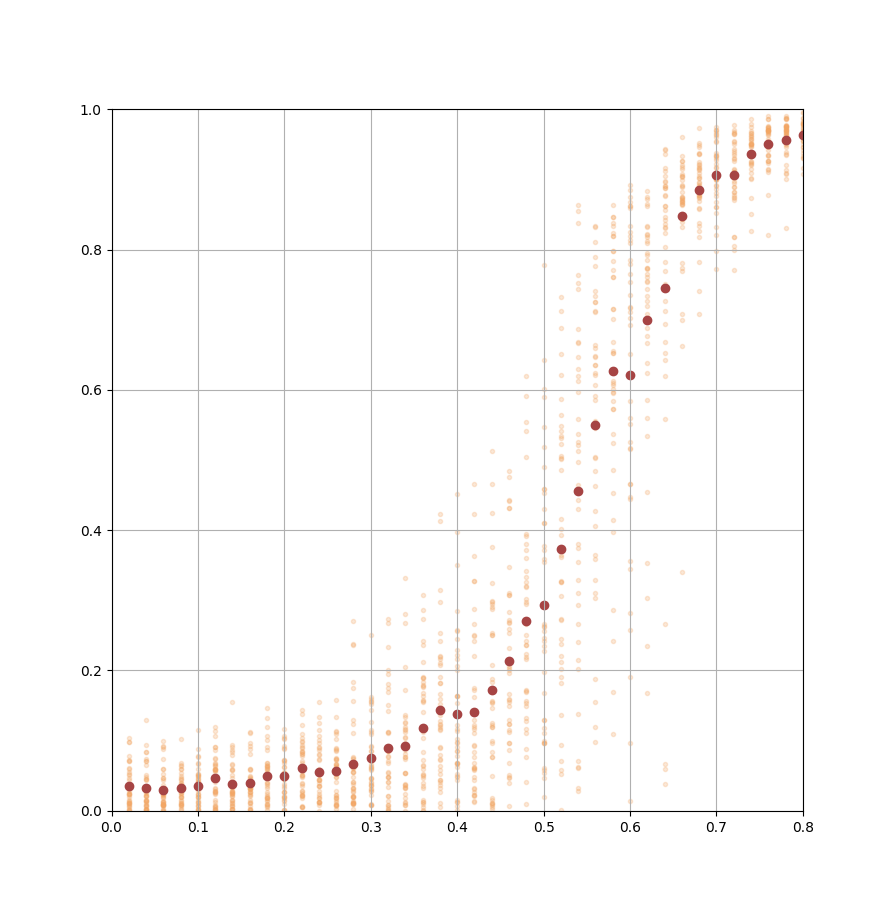
\includegraphics[width=\textwidth]{fortu_25}
\caption{Magnetizzazione in funzione di $\beta$ per $N=25$. Per ogni valore di
    $\beta$ sono stati fatti 40 campionamenti, rappresentati dai punti chiari. I
    punti scuri sono le medie.}
\label{fig:plot4}
\centering
\end{figure}

\begin{thebibliography}{9}
\bibitem{bremaud} 
Pierre Br\'emaud
\textit{Markov Chains, Gibbs Fields, Monte Carlo Simulation and Queues}. 
2020.
\bibitem{propp-wilson} 
James Gary Propp, David Bruce Wilson.
\textit{Exact Sampling with Coupled Markov Chains and Applications to Statistical
        Mechanics}. 
1996.
\bibitem{haggstrom} 
Olle H\"aggstr\"om
\textit{Finite Markov Chains and Algorithmic Applications}. 
2002.
\bibitem{edwards-sokal} 
Robert G. Edwards, Alan D. Sokal
\textit{Generalization of the Fortuin-Kasteleyn-Swendsen-Wang representation and
        Monte Carlo algorithm}. 
1988.
\end{thebibliography}

\end{document}
